\documentclass[../main.tex]{subfiles}
\begin{document}
In this chapter, we extend the data structure learned from the first part with more advanced data structures. These data structures are not as widely used as the basic data structures, however, they can be often seen to implement more advanced algorithms or they can be more efficient compared with algorithms that relies on a more basic version. 

%%%%%%%%%%%%%%%%%%%%%%%%%%%%%%%%%%%%%%%%%%%%%%%%%%%%%%%%%%%%%%%%%%%%%%%%%%%%%%%%%%%%%
%%%%%%%%%%%%% Monotonic Stack
%%%%%%%%%%%%%%%%%%%%%%%%%%%%%%%%%%%%%%%%%%%%%%%%%%%%%%%%%%%%%%%%%%%%%%%%%%%%%%%%%%%%%%%%%
\section{Monotone Stack}
\label{section_mono_stack}
\textit{A monotone Stack is a data structure the elements from the front to the end is strictly either increasing or decreasing. } For example, there is an line at the hair salo, and you would naturally start from the end of the line. However, if you are allowed to kick out any person that you can win at a fight, if every one follows the rule, then the line would start with the most powerful man and end up with the weakest one. This is an example of monotonic decreasing stack. 
\begin{itemize}
    \item Monotonically Increasing Stack: to push an element $e$, starts from the rear element, we pop out element $r>=e$ (violation); 
    \item Monotonically Decreasing Stack: we pop out element $r<=e$ (violation). T
\end{itemize}
The process of the monotone decresing stack is shown in Fig.~\ref{fig:mono_stack}.
\begin{figure}[h!]
    \centering
    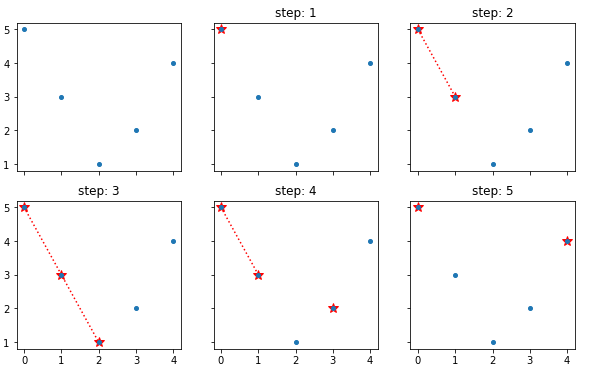
\includegraphics[width=0.9\columnwidth]{fig/monotone_stack_fig.png}
    \caption{The process of decreasing monotone stack}
    \label{fig:mono_stack}
\end{figure}
\textit{Sometimes, we can relax the strict monotonic condition, and can allow the stack or queue have repeat value. }

To get the feature of the monotonic queue, with $[5, 3, 1, 2, 4]$ as example, if it is increasing:
\begin{lstlisting}[numbers=none]
index   v   Increasing stack        Decreasing stack
1       5   [5]                     [5]
2       3   [3] 3 kick out 5        [5, 3] #3->5
3       1   [1] 1 kick out 3        [5, 3, 1] #1->3
4       2   [1, 2] #2->1            [5, 3, 2] 2 kick out 1
5       4   [1, 2, 4] #4->2         [5,4] 4 kick out 2, 3
\end{lstlisting}
By observing the above process, what features we can get? 
\begin{itemize}
    \item Pushing in to get smaller/larger item to the left: When we push an element in, if there exists one element right in front of it, 1) for increasing stack, we find the \textbf{nearest smaller item to the left} of current item, 2) for decreasing stack, we find the \textbf{nearest larger item} to the left instead. In this case, we get [-1, -1, -1, 1, 2], and [-1, 5, 3, 3, 5] respectively.
    \item Popping out to get smaller/larger item to the right: when we pop one element out, for the kicked out item, such as in step of 2, increasing stack, 3 forced 5 to be popped out, for 5, 3 is the first smaller item to the right. Therefore, if one item is popped out, for this item, the current item that is about to be push in is 1) for increasing stack, \textbf{the nearest smaller item to its right}, 2) for decreasing stack, \textbf{the nearest larger item to  its right}.  In this case, we get [3,1, -1, -1, -1], and [-1, 4, 2, 4, -1] respectively.
\end{itemize}
The conclusion is with monotone stack, we can search for smaller/larger items of current item either to its left/right. 

\paragraph{Basic Implementation}
 
This monotonic queue is actually a data structure that needed to add/remove element from the end. In some application we might further need to remove element from the front. Thus Deque from collections fits well to implement this data structure. Now, we set up the example data:
\begin{lstlisting}[language=Python]
A = [5, 3, 1, 2, 4]
import collections
\end{lstlisting}

\paragraph{Increasing Stack} We can find first smaller item to left/right.

\begin{lstlisting}[language=Python]
def increasingStack(A):
    stack = collections.deque()
    firstSmallerToLeft = [-1]*len(A)
    firstSmallerToRight = [-1]*len(A)
    for i,v in enumerate(A):
        while stack and A[stack[-1]] >= v: # right is from the popping out
            firstSmallerToRight[stack.pop()] = v  # A[stack[-1]] >= v 
        if stack:  #left is from the pushing in, A[stack[-1]] < v 
            firstSmallerToLeft[i] = A[stack[-1]]
        stack.append(i)
    return firstSmallerToLeft, firstSmallerToRight, stack
\end{lstlisting}
Now, run the above example with code:
\begin{lstlisting}[language=Python]
firstSmallerToLeft, firstSmallerToRight, stack = increasingQueue(A)
for i in stack:
    print(A[i], end = ' ')
print('\n')
print(firstSmallerToLeft)
print(firstSmallerToRight)
\end{lstlisting}
The output is:
\begin{lstlisting}
1 2 4 

[-1, -1, -1, 1, 2]
[3, 1, -1, -1, -1]
\end{lstlisting}

\paragraph{Decreasing Stack} We can find first larger item to left/right.

\begin{lstlisting}[language=Python]
def decreasingStack(A):
    stack = collections.deque()
    firstLargerToLeft = [-1]*len(A)
    firstLargerToRight = [-1]*len(A)
    for i,v in enumerate(A):
        while stack and A[stack[-1]] <= v:
            firstLargerToRight[stack.pop()] = v
            
        if stack:
            firstLargerToLeft[i] = A[stack[-1]]
        stack.append(i)
    return firstLargerToLeft, firstLargerToRight, stack
\end{lstlisting}
Similarily, the output is:
\begin{lstlisting}
5 4 

[-1, 5, 3, 3, 5]
[-1, 4, 2, 4, -1]
\end{lstlisting}
For the above problem, If we do it with brute force, then use one for loop to point at the current element, and another embedding for loop to look for the first element that is larger than current, which gives us $O(n^2)$ time complexity. If we think about the BCR, and try to trade space for efficiency, and use monotonic queue instead, we gain $O(n)$ linear time and $O(n)$ space complexity.  
% Let us look at an example, 
% \begin{lstlisting}
% Given an array [5, 3, 1, 2, 4], our target is to return an array of the same size that each element denotes the relative index we need to move to the right to find the first element that is larger than the current element, if we can not find, then we use -1. For this example the return would be  [-1, 3, 1, 1, -1].
% \end{lstlisting}


% Solution: If we do it with brute force, then use one for loop to point at the current element, and another embedding for loop to look for the first element that is larger than current, which gives us $O(n^2)$ time complexity. If we think about the BCR, and try to trade space for efficiency, we can use a decreasing monotonic queue. The first elment to the right that is larger than current is equaivalent to find the first element in the left that is smaller than the element(this means we need to use decreasing queue). First we have $[5]$, then $[5, 3]$, $[5, 3 ,1]$, then when $2$ comes in, we need to kick out $1$, so for $1$ the first larger element to its right size is $2$, we record $index(2)-index(1) = 1$. Then we have $4$, which could kick out $2$, so $4$ is the required one, then we set $r[index(2)] = index(4)-index(2) = 1$, then $r[index(3)] = index(4)-index(3) = 3$, Finally there would only $[5, 4]$, so we set them to be $-1$.
% \begin{lstlisting}
% index   v   decreasing queue
% 1       5   [5]
% 2       3   [5,3]
% 3       1   [5,3,1]
% 4       2   [5, 3, 2], kick out 1, we found the first larger number to the right of 1, which is 2
% 5       4   [5,4], kick out 2, for 2, we found 4, kick out 3, for 3 we found 4
% \end{lstlisting}
% \begin{lstlisting}[language = Python]
% a = [5, 3, 1, 2, 4]
% def firstLagerNumToRight(num):
%   if not num:
%     return []
%   monoStack = [] #decreasing monotonic stack
%   rst = [-1]*len(num)
%   for i, v in enumerate(num):
%     while  monoStack and v >= num[monoStack[-1]]:
%         index = monoStack.pop()
%         rst[index] = i-index
%     monoStack.append(i)
%   return rst
% print(firstLagerNumToRight(a))
% # [-1, 3, 1, 1, -1]
% \end{lstlisting}
Monotone stack is especially useful in the problem of subarray where we need to find smaller/larger item to left/right side of an item in the array. To better understand the features and applications of monotone stack, let us look at some examples. First, we recommend the audience to practice on these obvious applications shown in LeetCode Problem Section before moving to the examples:

There is one problem that is pretty interesting:

\paragraph{Sliding Window Maximum/Minimum } Given an array nums, there is a sliding window of size k which is moving from the very left of the array to the very right. You can only see the k numbers in the window. Each time the sliding window moves right by one position. Return the max sliding window. (LeetCode Probelm: 239. Sliding Window Maximum (hard))
\begin{lstlisting}[numbers=none]
Example:

Input: nums = [1,3,-1,-3,5,3,6,7], and k = 3
Output: [3,3,5,5,6,7] 
Explanation: 

Window position                Max
---------------               -----
[1  3  -1] -3  5  3  6  7       3
 1 [3  -1  -3] 5  3  6  7       3
 1  3 [-1  -3  5] 3  6  7       5
 1  3  -1 [-3  5  3] 6  7       5
 1  3  -1  -3 [5  3  6] 7       6
 1  3  -1  -3  5 [3  6  7]      7
\end{lstlisting}

\textbf{Analysis:} In the process of moving the window, any item that is smaller than its predecessor will not affect the max result anymore, therefore, we can use decrese stack to remove any trough. If the window size is the same as of the array, then the maximum value is the first element in the stack (bottom). With the sliding window, we record the max each iteration when the window size is the same as k. At each iteration, if need to remove the out of window item from the stack. For example of [5, 3, 1, 2, 4] with k = 3, we get [5, 3, 4]. At step 3, we get 5, at step 4, we remove 5 friom the stack, and we get 3. At step 5, we remove 3 if it is in the stack, and we get 4. With the monotone stack, we decrease the time complexity from $O(kn)$ to $O(n)$.
\begin{lstlisting}[language=Python]
import collections

def maxSlidingWindow(self, nums, k):
    ds = collections.deque()
    ans = []
    for i in range(len(nums)):
        while ds and nums[i] >= nums[ds[-1]]: indices.pop()
        ds.append(i)
        if i >= k - 1: ans.append(nums[ds[0]]) #append the current maximum
        if i - k + 1 == ds[0]: ds.popleft() #if the first also the maximum number is out of window, pop it out
    return ans
\end{lstlisting}

\begin{examples}[resume]
\item \textbf{907. Sum of Subarray Minimums (medium).} Given an array of integers A, find the sum of min(B), where B ranges over every (contiguous) subarray of A. Since the answer may be large, return the answer modulo $10^9 + 7$. \textit{Note: 1 <= A.length <= 30000, 1 <= A[i] <= 30000.}
\begin{lstlisting}[numbers=none]
Example 1:

Input: [3,1,2,4]
Output: 17
Explanation: Subarrays are [3], [1], [2], [4], [3,1], [1,2], [2,4], [3,1,2], [1,2,4], [3,1,2,4]. 
Minimums are 3, 1, 2, 4, 1, 1, 2, 1, 1, 1.  Sum is 17.
\end{lstlisting}

\textbf{Analysis:} For this problem, using naive solution to enumerate all possible subarries, we end up with $n^2$ subarray and the time complexity would be $O(n^2)$, and we will receive LTE. For this problem, we just need to sum over the minimum in each subarray. Try to consider the problem from another angel, what if we can figure out how many times each item is used as minimum value corresponding subarry? Then res = sum(A[i]*f(i)). If there is no duplicate in the array, then To get f(i), we need to find out:
\begin{itemize}
    \item left[i], the length of strict bigger numbers on the left of A[i],
    \item right[i], the length of strict bigger numbers on the right of A[i].
\end{itemize}
For the given examples, if A[i] = 1, then the left item is 3, and the right item is 4, we add 1*(left\_len*right\_len) to the result. However, if there is duplicate such as [3, 1, 4, 1], for the first 1, we need [3,1], [1], [1,4], [1, 4,1] with subarries, and for the second 1, we need [4,1], [1] instead. Therefore, we set the right length to find the >= item. Now, the problem in converted to the first smaller item on the left side and the first smaller or equal item on the right side. From the feature we draw above, we need to use increasing stack, as we know, from the pushing in, we find the first smaller item, and from the popping out, for the popped out item, the current item is the first smaller item on the right side. The code is as:
\begin{lstlisting}[language=Python]
def sumSubarrayMins(self, A):
    n, mod = len(A), 10**9 + 7
    left, s1 = [1] * n, []
    right = [n-i for i in range(n)]
    for i in range(n): # find first smaller to the left from pushing in
        while s1 and A[s1[-1]] > A[i]: # can be equal
            index = s1.pop()
            right[index] = i-index # kicked out
        if s1:
            left[i] = i-s1[-1]
        else:
            left[i] = i+1
        s1.append(i)
    return sum(a * l * r for a, l, r in zip(A, left, right)) % mod
\end{lstlisting}
The above code, we can do a simple improvement, by adding 0 to each side of the array. Then eventually there will only have [0, 0] in the stack. All of the items originally in the array they will be popped out, each popping, we can sum up the result directely:
\begin{lstlisting}[language=Python]
def sumSubarrayMins(self, A):
    res = 0
    s = []
    A = [0] + A + [0]
    for i, x in enumerate(A):
        while s and A[s[-1]] > x:
            j = s.pop()
            k = s[-1]
            res += A[j] * (i - j) * (j - k)
        s.append(i)
    return res % (10**9 + 7)
\end{lstlisting}
\end{examples}
\section{Disjoint Set}
\textbf{Disjoint-set data structure} (aka union-find data structure or merge-find set) maintains a collection $S = \{S_1, S_2, ..., S_k\}$ of disjoint \textit{dynamic} sets by partitioning a set of elements. We identify each set by a \textbf{representative}, which is some member of the set. It does matter which member is used only if we get the same answer both times if we ask for the representative twice without modifying the set. Choosing the smallest member in a set as representative is an examplary prespecified rule. According to its typical applications such as implementing Kruskal's minimum spanning tree algorithm and tracking connected components dynamically, disjoint-set should support the following operations:
\begin{enumerate}
    \item \texttt{make\_set(x)}: create a new set whose only member is $x$. To keep these sets to be disjoint, this member should not already be in some existent sets.
    \item \texttt{union(x, y)}: unites the two dynamic sets that contain $x$ and $y$, say $S_x \cup  S_y$ into a new set that is the union of these two sets. In practice, we merge one set into the other say $S_y$ into $S_x$, we then remove/destroy $S_y$. This will be more efficient than create a new one that unions and destroy the other two. 
    \item \texttt{find\_set(x)}: returns a pointer to the representative of the set that contains $x$.

\end{enumerate}
\paragraph{Applications} Disjoint sets are applied to implement union-find algorithm where perfoms \texttt{find\_set} and \texttt{union}. Union-find algorithms can be used into some basic graph algorithms, such as cycle detection, tracking connected components in the graph dynamically,  ~\footnote{where new edge will be added and the search based algorithm each time will be rerun to find them again}, Krauskal's MST algorithm, and Dijkstra's Shortest path algorithm.

\paragraph{Connected Component} Before we move to the implementation, let us first see how disjoint set can be applied to connected components.
\begin{figure}[h]
    \centering
    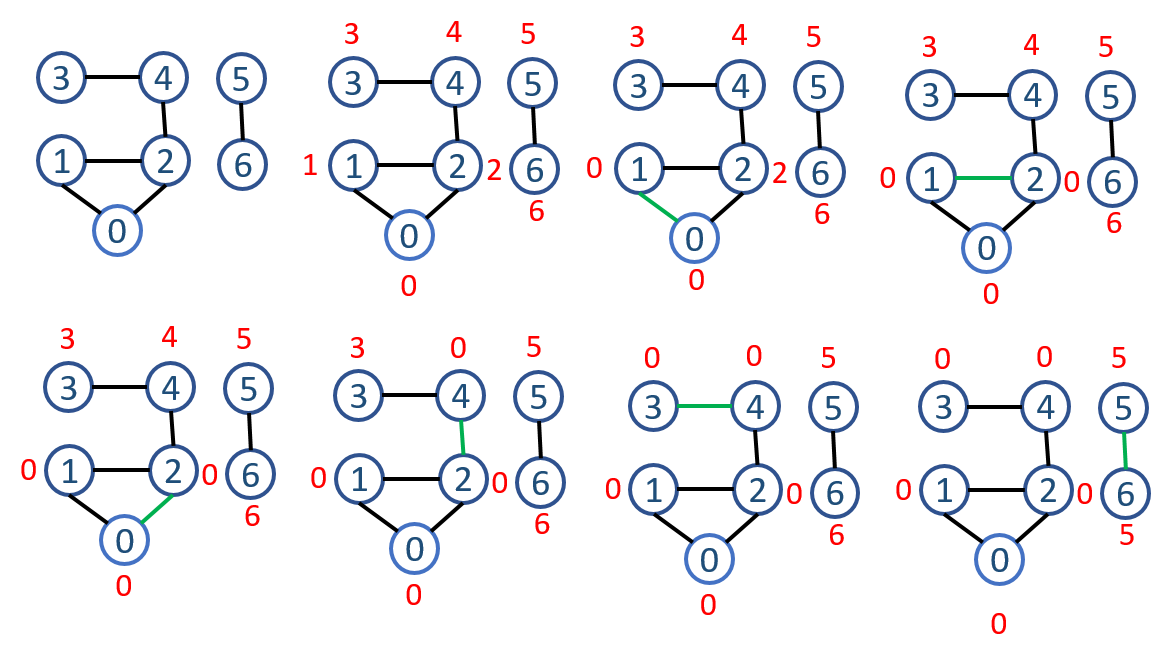
\includegraphics[width=0.98\columnwidth] {fig/disjoint_set.png}
    \caption{The connected components using disjoint set.}
    \label{fig:cc_undirected_disjoint_set}
\end{figure}
At first, we assign a set id for each vertex in the graph. Then we traverse each edge, and if the two endpoints of the edge belongs to different set, then we union the two sets. As shown in the process, first vertex 0 and 1 has different set id, then we update 1's id to 0. For edge (1, 2), we update 2's id to 0. For edge(0, 2), they are already in the same set, no update needed. We apply the same process with edge (2, 4), (3, 4), and (5, 6). 

\subsection{Basic Implementation with Linked-list or List}
Before we head off to more efficient and complex implementation, we first implement a baseline for the convenience of comparison. The key for the implementation is two dictionaries named \texttt{item\_set} (saves the mapping between item and its set id, which will only be one to one) and \texttt{set\_item} (the value of the key will be a list, because one set will have one to multiple relation). 

If our coding is right, each item must have an item when \texttt{find\_set} function is called, if not we will call \texttt{make\_set}. For each existing \texttt{set}, it will have at least one item. For function \texttt{union}, we choose the set that has less items to merge to the one that with more items. 

\begin{lstlisting}[language=Python]
class DisjointSet():
  '''Implement a basic disjoint set'''
  def __init__(self, items):
    self.n = len(items)
    self.item_set = dict(zip(items, [i for i in range(self.n)])) # first each set only has one item [i], this can be one->multiple match
    self.set_item = dict(zip([i for i in range(self.n)], [[item] for item in items])) # each item will always belong to one set
    
  def make_set(self, item):
    '''make set for new incoming set'''
    if item  in self.item_set:
      return
    
    self.item_set[item] = self.n
    self.n += 1
    
  def find_set(self, item):
    if item in self.item_set:
      return self.item_set[item]
    else:
      print('not in the set yet: ', item)
      return None
    
  def union(self, x, y):
    id_x = self.find_set(x)
    id_y = self.find_set(y)
    if id_x == id_y:
      return
    
    sid, lid = id_x, id_y
    if len(self.set_item[id_x]) > len(self.set_item[id_y]):
      sid, lid = id_y, id_x
    # merge items in sid to lid 
    for item in self.set_item[sid]:
      self.item_set[item] = lid
    self.set_item[lid] += self.set_item[sid]
    del self.set_item[sid]
    return 
\end{lstlisting}

\paragraph{Complexity} For $n$ items, we spend $O(n)$ time to initialize the two hashmaps. With the help of hashmap, function \texttt{find\_set} tasks only $O(1)$ time, accumulating it will give us $O(n)$. For function \texttt{union}, it takes more effort to analyze. From another angle, for one item $x$, it will only update its item id when we are unioning it to another set $x_1$. The first time, the resulting set $x_1$ will have at least two items. The second update will be union $x_1$ to $x_2$. Because the merged one will have smaller length, thus the resulting items in $x_2$ will at least be 4. Then it is the third, ..., up to $k$ updates. Because a resulting set will at most has $n$ in size, so for each item, at most $\log n$ updates will be needed. For $n$ items, this makes the upper bound for \texttt{union} to be $n\log n$. 

However, for our implementation, we has additional cost, which is in \texttt{union}, where we merge the list. This cost can be easily limited to constant by using linked list. However, even with \texttt{list}, there are different ways to concatenate one list to another:

\begin{enumerate}
\item Use $+$ operator: The time complexity of the concat operation for two lists, A and B, is O(A + B). This is because you aren't adding to one list, but instead are creating a whole new list and populating it with elements from both A and B, requiring you to iterate through both.

\item \texttt{extend(lst)}: Use extend which doesn't create a new list but adds to the original. The time complexity should only be $O(1)$. On the other hand \texttt{l += [i]} modifies the original list and behaves like extend.
\end{enumerate}

\subsection{Implementation with Disjoint-set Forests}
Instead of using linear linked list, we use tree structure. Different with trees we have introduced before that a node points to its children, an item here will only points to its parent. A tree represents a set, and the root node is the representative and it points to itself. The straightforward algorithms that use this structure are not faster than the linked-list version. By introducing two heuristics--``Union by rank'' and ``path compression"--we can achieve asympotically optimal disjoint-set data structure.
\begin{figure}[h]
    \centering
    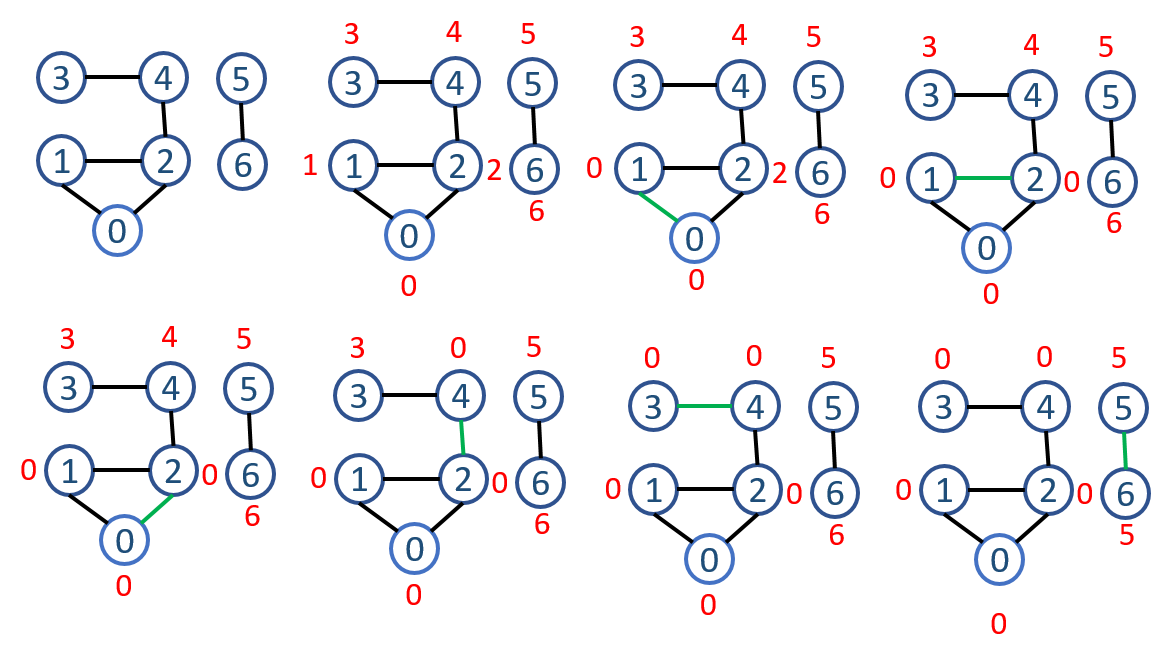
\includegraphics[width=0.98\columnwidth] {fig/disjoint_set.png}
    \caption{A disjoint forest}
    \label{fig:disjoint_forest_1}
\end{figure}
\subsubsection{Naive Version} We first need to create a \texttt{Node} class which stores \texttt{item} and another parent pointer \texttt{parent}. An \texttt{item} can be any immutable data structure with necessary information represents a node.
\begin{lstlisting}[language=Python]
class Node:
  def __init__(self, item):
    self.item = item # save node information
    self.parent = None
\end{lstlisting}

We need one dict data structure \texttt{item\_finder} and one set data structure \texttt{sets} to track nodes and set. From \texttt{item\_finder} we can do (item, node) map to find node, and then from the node further we can find its set representative node or execute \texttt{union} operation. \texttt{sets} is used to track all the representative nodes. When we union two sets, the one merged to the other will be deleted in \texttt{sets}. At the easy version, \texttt{make\_set} will create  tree with only one node. \texttt{find\_set} will start from the node and traverse all the way back to its final parent which is when \texttt{node.parent==node}. And a \texttt{union} operation will simply point one tree's root node to the root of another through \texttt{parent}. The code is as follows:
\begin{lstlisting}[language=Python]
class DisjointSet():
  '''Implement with disjoint-set forest'''
  def __init__(self, items):
    self.n = len(items)
    self.item_finder = dict()
    self.sets = set() # sets will have only the parent node
    
    for item in items:
      node = Node(item)
      node.parent = node
      self.item_finder[item] = node # from item we can find the node
      self.sets.add(node)
    
  def make_set(self, item):
    '''make set for new incoming set'''
    if item  in self.item_finder:
      return
    
    node = Node(item)
    node.parent = node
    self.item_finder[item] = node
    self.sets.add(node)
    self.n += 1
    
  def find_set(self, item):
    # from item->node->parent to set representative
    if item not in self.item_finder:
      print('not in the set yet: ', item)
      return None
    node = self.item_finder[item]
    while node.parent != node:
      node = node.parent
    return node
    
  def union(self, x, y):
    node_x = self.find_set(x)
    node_y = self.find_set(y)
    if node_x.item == node_y.item:
      return
    
    #the root of one tree to point to the root of the other
    # merge x to y
    node_x.parent = node_y
    #remove one set
    self.sets.remove(node_x)
    return 
  
  def __str__(self):
    ans = ''
    for root in self.sets:
      ans += 'set: '+ str(root.item) + '\n'
    return ans
  
  def print_set(self, item):
    if item in self.item_finder:
      node = self.item_finder[item]
      print(node.item, '->', end='')
      while node.parent != node:
        node = node.parent
        print(node.item, '->', end='')
\end{lstlisting}
Let's run an example:
\begin{lstlisting}[language=Python]
ds = DisjointSet(items=[i for i in range(5)])
ds.union(0,1)
ds.union(1,2)
ds.union(2,3)
ds.union(3, 4)
print(ds)
for item in ds.item_finder.keys():
  ds.print_set(item)
  print(' ')
\end{lstlisting}
The output is:
\begin{lstlisting}[numbers=none]
set: 4

0 ->1 ->2 ->3 ->4 -> 
1 ->2 ->3 ->4 -> 
2 ->3 ->4 -> 
3 ->4 -> 
4 -> 
\end{lstlisting}
The above implementation, both \texttt{make\_set} and \texttt{union} takes $O(1)$ time complexity. The main time complexity is incurred at \texttt{find\_set}, which traverse a path from node to root. If we assume each tree in the disjoint-set forest is balanced, the upper bound of this operation will be $O(\log n)$. However, if the tree is as worse as a linear linked list, the time complexity will goes to $O(n)$. This makes the total time complexity from $O(n\log n)$ to $O(n^2)$. 

\subsubsection{Heuristics}
\paragraph{Union by Rank}
As we have seen from the above example, A sequence of $n-1$ \texttt{union} operations may create a tree that is just a linear chain of $n$ nodes. Union by rank, which is similar to the weighted-union heuristic we used with the linked list implementation, is applied to avoid the worst case.  For each node, other than the parent pointer, it adds \texttt{rank} to track the upper bound of the height of the associated node (the number of edges in the longest simple path between the node and a descendant leaf). In union by rank, we make the root with smaller rank point to the root with larger rank. 

In the initialization, and \texttt{make\_set} operation, a single noded tree has an initial rank of 0. In \texttt{union(x, y)}, there will exist three cases:
\begin{lstlisting}[numbers=none]
Case 1 x.rank == y.rank: 
        join x to y
        y.rank += 1
Case 2: x.rank < y.rank:
       join y to x
       x.rank += 1
Case 3: x.rank > y.rank:
        join y to x
        x's rank stay unchanged
\end{lstlisting}
Now, with adding \texttt{rank} to the node. We modify the naive implementation:
\begin{lstlisting}[language=Python]
class Node:
  def __init__(self, item):
    self.item = item # save node information
    self.parent = None
    self.rank = 0
\end{lstlisting}
The updated implementation of \texttt{union}:
\begin{lstlisting}[language=Python]
  def union(self, x, y):
    node_x = self.find_set(x)
    node_y = self.find_set(y)
    if node_x.item == node_y.item:
      return
    
    # link
    if node_x.rank > node_y.rank:
      node_y.parent = node_x
      #remove one set
      self.sets.remove(node_y)
    elif node_x.rank < node_y.rank:
      node_x.parent = node_y
      self.sets.remove(node_x)
    else:
      node_x.parent = node_y
      node_y.rank += 1
      self.sets.remove(node_x)
    return 
\end{lstlisting}

\paragraph{Path Compression}
In our naive implementation, \texttt{find\_set} took the most time. With path compression, during the process of \texttt{find\_set}, it simply make each node on the find path point directly to its root. Path Compression wont affect the rank of each node. Now, we modify this function:
\begin{lstlisting}[language=Python]
  def _find_parent(self, node):
    while node.parent != node:
      node = node.parent
    return node
    
  def find_set(self, item):
    '''modified to do path compression'''
    # from item->node->parent to set representative
    if item not in self.item_finder:
      print('not in the set yet: ', item)
      return None
    node = self.item_finder[item]
    node.parent = self._find_parent(node) # change node's parent to the root node
    return node.parent
\end{lstlisting}
The same example, the output will be:
\begin{lstlisting}[numbers=none]
set: 1

0 ->1 -> 
1 -> 
2 ->1 -> 
3 ->1 -> 
4 ->1 ->
\end{lstlisting}
\begin{lstlisting}[language=Python]
import time, random
t0 =  time.time()
n = 100000
ds = DisjointSet(items=[i for i in range(n)])
for _ in range(n):
  i, j = random.randint(0, n-1), random.randint(0, n-1) #[0,n]
  ds.union(i, j)
print('time: ', time.time()-t0)
\end{lstlisting} 
\begin{bclogo}[couleur = blue!30, arrondi=0.1,logo=\bccrayon,ombre=true]{Experiment to the running time of Linked-list VS naive forest VS heuristic forest} We run the disjoint set with n=100,000, and with n times of union: 
\begin{lstlisting}[language=Python]
import time, random
t0 =  time.time()
n = 100000
ds = DisjointSet(items=[i for i in range(n)])
for _ in range(n):
  i, j = random.randint(0, n-1), random.randint(0, n-1) #[0,n]
  ds.union(i, j)
print('time: ', time.time()-t0)
\end{lstlisting}
The resulting time is: 1.09s, 50.4s, 1.19s
\end{bclogo}
\paragraph{Note} As we see, in our implementation, we have never removed any item from disjoint-set structure. Also, from the above implementation, we know the sets of the nodes, but we cant track items from the root node. How can we further improve this?
\section{Fibonacci Heap}
\section{Exercises}
\subsection{Knowledge Check}
\subsection{Coding Practice}
\paragraph{Disjoint Set}
\begin{enumerate}
    \item 305. Number of Islands II (hard)
\end{enumerate}
\end{document}